\section{Les choses se GATT}

\begin{frame}
	\frametitle{Stack BLE}
	\begin{minipage}{0.45\linewidth}
		\begin{figure}
			\includegraphics[height=6cm]{img/HCI_GATT.png}
		\end{figure}
	\end{minipage}
	\begin{minipage}{0.50\linewidth}
		\begin{block}{Stack Bluetooth Low Energy}
			\begin{itemize}
				\item Link Layer
				\item L2CAP
				\item Protocole ATT
				\item Profile GATT
				\item Services : Application
			\end{itemize}
		\end{block}
	\end{minipage}
\end{frame}

\begin{frame}
	\frametitle{Link Layer}
\end{frame}

\begin{frame}
	\frametitle{ATT}
	\begin{quote}A protocol for discovering, reading, and writing attributes on a peer device.\end{quote}

	\begin{block}{\textbf{ATT}ribute}
		\begin{itemize}
			\item Type : UUID
			\item Handle : 16 bit
			\item Permissions :
				\begin{itemize}
					\item Lecture / Écriture
					\item Notification
					\item Encryption
					\item Autorisation
					\item Authentification
				\end{itemize}
		\end{itemize}
	\end{block}
\end{frame}

\begin{frame}
	\frametitle{GATT}
	\center{\textbf{G}eneric \textbf{ATT}ribute Profile}
	\begin{figure}
		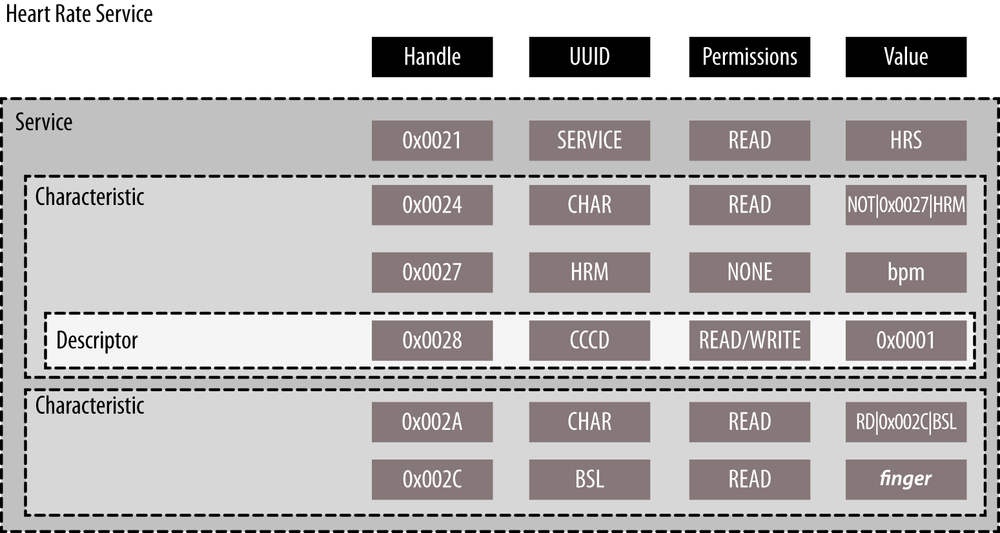
\includegraphics[height=5cm]{img/gatt.png}
	\end{figure}
{\tiny "Getting started with bluetooth low energy", R.Davidson, Akiba, Carles Cufí, Kevin Townsend, O'Reilly}

\end{frame}

\begin{frame}
	\frametitle{Exemple de service}
\end{frame}
